\documentclass[xcolor=pdflatex,dvipsnames,table]{beamer}
\usepackage{epsfig,graphicx}
\usepackage{palatino}
\usepackage{fancybox}
\usepackage{relsize}
\usepackage[procnames]{listings}
\usepackage{hyperref}
\usepackage{qtree} % needed?
\usepackage{booktabs}
\usepackage{dirtree}
\usepackage[normalem]{ulem}


% fatter TT font
\renewcommand*\ttdefault{txtt}
% another TT, suggested by Alex
% \usepackage{inconsolata}
% \usepackage[T1]{fontenc} % needed as well?


\newcommand{\scale}{0.7}

\newcommand{\todo}[1]{{\emph{TODO: #1}}}
\newcommand{\martin}[1]{{\color{blue} Martin: #1}}
\newcommand{\abcdef}[1]{{\color{red} Author2: #1}}

% uncomment following for final submission
%\renewcommand{\todo}[1]{}
%\renewcommand{\martin}[1]{}
%\renewcommand{\author2}[1]{}

\newcommand{\code}[1]{{\texttt{#1}}}

\hypersetup{
  linkcolor  = black,
%  citecolor  = blue,
  urlcolor   = blue,
  colorlinks = true,
}

\beamertemplatenavigationsymbolsempty
\setbeamertemplate{footline}[frame number]





\newif\ifbook
% shared in slides and book

\lstdefinelanguage{chisel}{
%  morekeywords={abstract,case,catch,class,def,%
%    do,else,extends,false,final,finally,%
%    for,if,implicit,import,match,mixin,%
%    new,null,object,override,package,%
%    private,protected,requires,return,sealed,%
%    super,this,throw,trait,true,try,%
%    type,val,var,while,with,yield},
%  otherkeywords={=>,<-,<\%,<:,>:,\#,@},
  sensitive=true,
  morecomment=[l]{//},
  morecomment=[n]{/*}{*/},
  morestring=[b]",
  morestring=[b]',
  morestring=[b]"""
}

\usepackage{color}
\definecolor{dkgreen}{rgb}{0,0.6,0}
\definecolor{gray}{rgb}{0.5,0.5,0.5}
\definecolor{mauve}{rgb}{0.58,0,0.82}

% Default settings for code listings
%\ifbook
\lstset{%frame=lines,
  language=chisel,
  aboveskip=3mm,
  belowskip=3mm,
  showstringspaces=false,
  columns=fixed, % basewidth=\mybasewidth,
  basicstyle={\small\ttfamily},
  numbers=none,
  numberstyle=\footnotesize,
  % identifierstyle=\color{red},
  breaklines=true,
  breakatwhitespace=true,
  procnamekeys={def, val, var, class, trait, object, extends},
  % procnamestyle=\ttfamily,
  tabsize=2,
  float
}
%\else
%\lstset{%frame=lines,
%  language=chisel,
%  aboveskip=3mm,
%  belowskip=3mm,
%  showstringspaces=false,
%  columns=fixed, % basewidth=\mybasewidth,
%  basicstyle={\small\ttfamily},
%  numbers=none,
%  numberstyle=\footnotesize\color{gray},
%  % identifierstyle=\color{red},
%  keywordstyle=\color{blue},
%  commentstyle=\color{dkgreen},
%  stringstyle=\color{mauve},
%  breaklines=true,
%  breakatwhitespace=true,
%  procnamekeys={def, val, var, class, trait, object, extends},
%  procnamestyle=\ttfamily\color{red},
%  tabsize=2,
%  float
%}
%\fi

\lstnewenvironment{chisel}[1][]
{\lstset{language=chisel,#1}}
{}

\newcommand{\shortlist}[1]{{\lstinputlisting[nolol]{#1}}}

\newcommand{\longlist}[3]{{\lstinputlisting[float, caption={#2}, label={#3}, frame=tb, captionpos=b]{#1}}}

\newcommand{\verylonglist}[3]{{\lstinputlisting[caption={#2}, label={#3}, frame=tb, captionpos=b]{#1}}}


\title{The Vending Machine}
\author{Martin Schoeberl}
\date{\today}
\institute{Technical University of Denmark\\
Embedded Systems Engineering}

\begin{document}

\begin{frame}
\titlepage
\end{frame}


\begin{frame}[fragile]{Overview}
\begin{itemize}
\item Your final grade
\item Online exam
\item GoL in hardware
\item The Vending Machine project
\item
\item How did it go with the UART?
\end{itemize}
\end{frame}

\begin{frame}[fragile]{Your Final Grade}
\begin{enumerate}
\item Your lab work, the vending machine
\begin{itemize}
\item What is working (TA checks)
\item Your report
\item Basic functions is a 7, extra functions needed for a 10 or 12
\end{itemize}
\item Written exam
\begin{itemize}
\item Two hour written exam
\end{itemize}
\end{enumerate}
\end{frame}

\begin{frame}[fragile]{Exam Topics and Questions}
\begin{itemize}
\item The pensum (reading lis) is on the \href{http://www2.imm.dtu.dk/courses/02139/}{web site}
\item Compute maximum frequency and delays of a given circuit
\item Given a Chisel description of a circuit, draw it
\item Given a circuit drawing, sketch the Chisel description
\item Basically what we have done in the lab
\item No surprises (at least not too many ;-)
\end{itemize}
\end{frame}

\begin{frame}[fragile]{Game of Live}
\begin{itemize}
\item \href{https://en.wikipedia.org/wiki/Conway\%27s_Game_of_Life}{Conway's Game of Life}
\item Any live cell with two or three live neighbors survives.
\item Any dead cell with three live neighbors becomes a live cell.
\item All other live cells die in the next generation. Similarly, all other dead cells stay dead.
\end{itemize}
\end{frame}

\begin{frame}[fragile]{Game of Live}
\begin{itemize}
\item You did an implementation in Java
\item The problem is highly parallel
\item I will show you a Chisel (and Java) implementation
\item FPGA version is extremely fast compared to the Java implementation
\item \url{https://github.com/schoeberl/game-of-live}
\end{itemize}
\end{frame}

\begin{frame}[fragile]{Performance Comparison}
\begin{table}
  \centering
\begin{tabular}{crrrrrr}
    \toprule
    & &\multicolumn{3}{c}{Execution time (us)} & \multicolumn{2}{c}{FPGA Speedup}\\
World & Cells&Mac&Rasperry&FPGA& Mac& Rasperry\\
\midrule
10x10 & 100&0.10&1.783&0.0040&25&445\\
20x20 & 400&0.33&5.137&0.0040&82&1284\\
30x30 & 900&0.70&9.965&0.0041&170&2430\\
40x40 & 1600&1.21&17.212&0.0040&302&4302\\
50x50 & 2500&1.81&25.204&0.0044&411&5728\\
60x60 & 3600&2.76&37.822&0.0045&613&8404\\
70x70 & 4900&3.54&57.665&0.0040&884&14416\\
80x80 & 6400&4.81&64.396&0.0047&1023&13701\\
90x90 & 8100&6.50&81.309&0.0045&1444&18068\\
100x100 & 10000&7.51&109.964&0.0048&1564&22909\\
\bottomrule
\end{tabular}
    \label{tab:speedup}
\end{table}
\end{frame}

\begin{frame}[fragile]{A Vending Machine from 1952}
\begin{figure}
    \centering
    \href{https://en.wikipedia.org/wiki/File:CandiesVendingMachine1952.jpg}{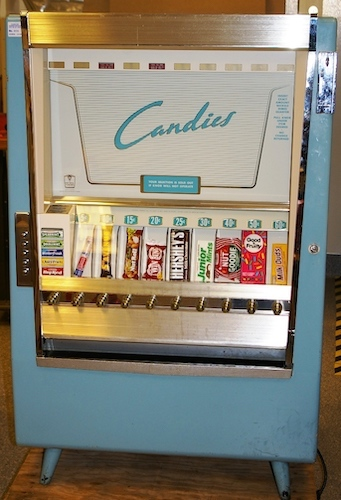
\includegraphics[scale=0.4]{CandiesVendingMachine1952}}

\end{figure}

{\tiny Source: Minnesota Historical Society, \href{https://creativecommons.org/licenses/by-sa/2.0}{CC BY-SA 2.0}}
\end{frame}

\begin{frame}[fragile]{The Vending Machine}
\begin{itemize}
\item Final project is a vending machine
\item Description is on GitHub: \href{https://github.com/schoeberl/chisel-lab/tree/master/vending}{README.md}
\item Will repeat the overview now
\item Group work
\item Final version shall be run in an FPGA
\item A lot can be done with testing and simulation
\end{itemize}
\end{frame}

\begin{frame}[fragile]{The Vending Machine}
\begin{itemize}
\item Inputs: coins, buy
\item Display: price and current amount
\item Output: release can or error
\item Small challenge to multiplex the display
\item State machine with data path is the \emph{brain} of the VM
\item Guided step by step over several weeks
\end{itemize}
\end{frame}

\begin{frame}[fragile]{Vending Machine Specification I}
\begin{itemize}
\item Sell 1 item and not returning any money
\item Set price with 5 switches (1--31 kr.)
\item Display price on two 7-segment displays (hex.)
\item Accept 2 and 5 kr. (two push buttons)
\item Display sum on two 7-segment displays (hex.)
\begin{itemize}
\item Amount entered so far
\end{itemize}
\item Does not return money, left for the next purchase
\end{itemize}
\end{frame}

\begin{frame}[fragile]{Vending Machine Specification II}
\begin{itemize}
\item Push button \emph{Buy}
\begin{itemize}
\item If not enough money, activate \emph{alarm} as long as buy is pressed
\item If enough money, activate \emph{release item} for as long as \emph{buy}
is pressed and reduce \emph{sum} by the price of the item
\end{itemize}
\end{itemize}
\end{frame}

\begin{frame}[fragile]{Optional Extras}
\begin{itemize}
\item Needed for a 10 or 12
\item Display decimal numbers
\item Supplement alarm by some visuals (e.g., blinking display)
\item Count coins and display an alarm when compartment is full ($>$ 20 coins)
\item Have some text scrolling on the display
\item Connect a UART to your VM and sending messages to your laptop
\item ...
\item Your ideas :-)
\end{itemize}
\end{frame}

\begin{frame}[fragile]{Design and Implementation}
\begin{itemize}
\item Implementation shall be a state machine plus datapath
\item Design your datapath on a sheet of paper
\item Datapath
\begin{itemize}
\item Does add and subtract
\item Contains a register to hold the sum
\item Needs some multiplexer to operate
\end{itemize}
\item Display needs multiplexing
\begin{itemize}
\item Implemented with some counters and a multiplexer
\end{itemize}
\item Show each part of your design to a TA
\begin{itemize}
\item 7-segment decoder, 7-segment with a counter, display multiplexer, complete vending machine
\end{itemize}
\end{itemize}
\end{frame}

\begin{frame}[fragile]{Draw Figures}
\begin{itemize}
\item Drawings/schematics is another language to describe (digital) circuits
\item Draw, draw, draw boxes and arrows!
\item Use drawing during development
\item If you cannot draw your circuit you do not understand it
\item Use drawings to communicate with the TA
\item Have drawings in your report
\item You will \emph{for sure} need to draw circuits at the exam ;-)
\end{itemize}
\end{frame}


\begin{frame}[fragile]{Vending Machine Design and Implementation Steps}
\begin{itemize}
\item We started in week 6 (now we are in week 10)
\item lab 6: Hexadecimal to 7-segment decoder and counter
\item lab 8: Multiplexed Seven-Segment Display
\item lab 10--13: Complete Vending Machine
\item \emph{Show your working design to a TA}
\end{itemize}
\end{frame}

\begin{frame}[fragile]{Final Report}
\begin{itemize}
\item One report per group
\item A single PDF
\begin{itemize}
\item Your group number is part of the file name (e.g., group7.pdf)
\item Code as listing in an appendix (no .zip files)
\item Hand in in DTU Inside
\end{itemize}
\item Content
\begin{itemize}
\item Abstract
\item Preface (Who did what)
\end{itemize}
\begin{enumerate}
\item Introduction and Problem Formulation
\item Analysis and Design
\item Implementation
\item Testing
\item Results
\item Discussion
\item Conclusion
\end{enumerate}
\begin{itemize}
\item List of References
\item Appendix: Chisel code
\end{itemize}
\end{itemize}
\end{frame}

\begin{frame}[fragile]{Material on the Lab GitHub}
\begin{itemize}
\item A top-level component
\item XDC file for Basys pins and frequency
\item A start of a tester generating waveforms
\item A simulation of the board
\item Show it (in IntelliJ)
\end{itemize}
\end{frame}

\begin{frame}[fragile]{An Optional Lab}
\begin{itemize}
\item Testing the a Vending Machine
\item Black box testing (you don't see the implementation)
\item I give you two implementations
\item One is OK, one is broken
\item Which one is broken, and what it the error?
\item Issue is that you need Verilator and a C compiler to run the tests
\item Therefore, only if you really want to do it
\item \href{https://github.com/schoeberl/chisel-lab/tree/master/lab10}{Lab 10}
\end{itemize}
\end{frame}


\begin{frame}[fragile]{Questions on Final Project?}
\end{frame}


\begin{frame}[fragile]{Summary}
\begin{itemize}
\item Now you have four weeks for the Vending Machine
\item Should be plenty of time
\item Standard solution is good for a standard grade
\item Add features as you like
\item Have a good time with your Vending Machine construction
\end{itemize}
\end{frame}



\end{document}

%\begin{frame}[fragile]{xxx}
%\begin{itemize}
%\item yyy
%\end{itemize}
%\end{frame}
